\begin{EXO}{Modélisation d'une évolution de poids}{}
Une personne s'est pesée toutes les semaines pendant un an en 2018. Sa courbe de poids peut être modélisée par une fonction polynôme de degré 2 dont l'expression est $f(x)=0.008x^2-0.4x+75$ où $x$ correspond au temps en semaines à partir du premier janvier 2018 ($x\in \CrochetG0;52\CrochetD$).
\begin{tcbenumerate}[2]
\tcbitem \tcbitempoint{3} Dresser le tableau de variations de la fonction $f$.
\setrdcrep{seyes=false,correction color=black,correction font=\normalsize}
\begin{crep}[colback=white,colframe=white]
Forme canonique : $f(x) = 0{,}008(x-25)^2 + 70$\\\\

\begin{tikzpicture}
\tkzTabInit{$x$/1,$f$/1.8}
{$0$,$25$,$52$}
\tkzTabVar{+/$75$,-/$70$,+/$75{,}632$}
\end{tikzpicture}
\end{crep}

\tcbitem[colframe=black,boxrule=0.4pt] En utilisant cette modélisation, répondre aux questions suivantes.
\begin{tcbenumerate}[2][1][alph]
\tcbitem \tcbitempoint{1} Quel était son poids maximal sur l'année ? Quand a-t-il été atteint ?

\begin{crep}
Poids maximal : $75{,}632$ kg atteint à la semaine $52$
\end{crep}

\tcbitem \tcbitempoint{1} Quel était son poids minimal sur l'année ? Quand a-t-il été atteint ?

\begin{crep}
Poids minimal : $70$ kg atteint à la semaine $25$
\end{crep}
\end{tcbenumerate}
\end{tcbenumerate}

\exocorrection

\begin{tcbenumerate}[2]
\tcbitem Pour dresser le tableau de variations, déterminons la forme canonique :

$f(x) = 0{,}008x^2 - 0{,}4x + 75$

$\alpha = -\dfrac{b}{2a} = -\dfrac{-0{,}4}{2 \times 0{,}008} = \dfrac{0{,}4}{0{,}016} = 25$

$\beta = f(25) = 0{,}008 \times 25^2 - 0{,}4 \times 25 + 75 = 5 - 10 + 75 = 70$

Donc $f(x) = 0{,}008(x-25)^2 + 70$.

Comme $a = 0{,}008 > 0$, la parabole est tournée vers le haut.

Sur $\CrochetG0;52\CrochetD$ : minimum en $x = 25$ avec $f(25) = 70$.

Aux bornes : $f(0) = 75$ et $f(52) = 0{,}008 \times 27^2 + 70 = 5{,}832 + 70 = 75{,}632$

\tcbitem D'après le tableau de variations :
\begin{tcbenumerate}[2]
\tcbitem Le poids maximal est $75{,}632$ kg, atteint à la fin de l'année (semaine 52).
\tcbitem Le poids minimal est $70$ kg, atteint à la semaine 25 (fin juin).
\end{tcbenumerate}
\end{tcbenumerate}
\end{EXO}